% ============================================================
\section{Resultados del Entregable~1}
\label{sec:resultados}
% ============================================================

Del universo de 102 modelos CMIP6 que publican \texttt{tos}/\texttt{Omon} en ESGF, 40 completaron los cuatro experimentos requeridos y aprobaron el control de calidad final: 160 combinaciones modelo-experimento, todas con estado \texttt{PASS}. El Cuadro~\ref{tab:cuentas} resume cómo se llega a esa cifra.

\begin{table}[htbp]
\centering
\caption{Del universo de modelos candidatos al conjunto seleccionado.}
\label{tab:cuentas}
\small
\begin{tabular}{@{}L{9.6cm}rL{\dimexpr\textwidth-9.6cm-1.2cm-6\tabcolsep\relax}@{}}
\toprule
\textbf{Conjunto} & \textbf{Modelos} & \textbf{Fuente} \\
\midrule
Publican \texttt{tos}/\texttt{Omon} en ESGF (universo) & 102 & Paso~00b \\
Publican \texttt{historical}, \texttt{ssp245} y \texttt{ssp585} & 49 & Paso~00b \\
Publican además \texttt{ssp370} (lista de descarga) & 41 & Paso~00b \\
Completos y aprobados en el control de calidad (seleccionados) & 40 & Pasos~06--07 \\
\midrule
Excluidos: algún experimento no disponible en ninguna fuente consultada & 44 & Pasos~00b--02 \\
Excluidos: disponibilidad o descarga incompleta & 18 & Pasos~00b--02 \\
\bottomrule
\end{tabular}
\end{table}

La Figura~\ref{fig:qc} muestra el estado de cada modelo y experimento para el universo completo. Cada celda toma uno de seis estados: aprobado (el archivo se descargó y pasó el control de calidad); rechazado (se descargó pero no lo pasó); descarga pendiente (existe un enlace de descarga activo pero el archivo aún no se descargó o procesó); sin enlace (el Paso~00b encontró el experimento, pero el Paso~01 no encontró ningún enlace activo); solo \texttt{hist-1950} (el modelo publica la variante HighResMIP 1950--2014 en lugar de \texttt{historical}; estos modelos no corren los SSP estándar y nunca reúnen los cuatro experimentos); y no disponible (el experimento no existe en ningún nodo consultado). En la corrida final no quedó ningún archivo rechazado.

\begin{figure}[htbp]
\centering
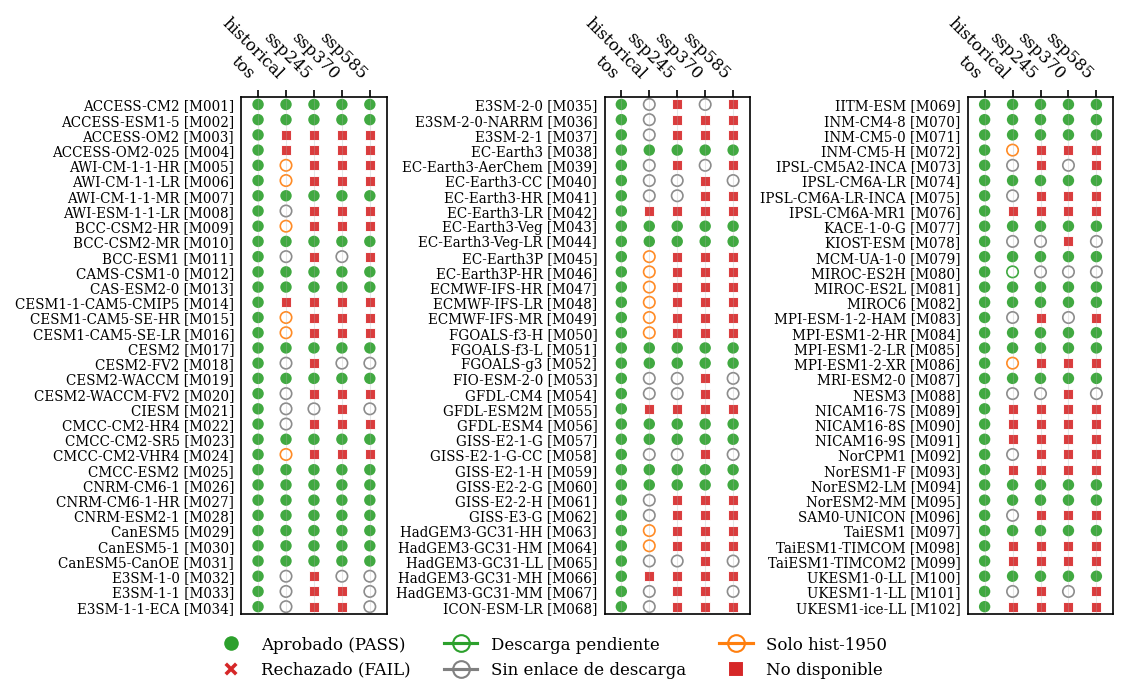
\includegraphics[width=\textwidth]{figuras/sst_QD_vf.png}
\caption[Disponibilidad y control de calidad de \texttt{tos}/\texttt{Omon} para los 102 modelos candidatos.]{Estado por modelo (nombre y código \texttt{M001}--\texttt{M102}) y por columna (\texttt{tos}, \texttt{historical}, \texttt{ssp245}, \texttt{ssp370}, \texttt{ssp585}) para los 102 modelos candidatos. Los 40 modelos seleccionados son los que tienen las cinco columnas aprobadas.}
\label{fig:qc}
\end{figure}

Como verificación exploratoria de la homogeneización, se compara ERSSTv5 con tres de los nueve modelos seleccionados de resolución nominal más gruesa, 250\,km: ACCESS-CM2, ACCESS-ESM1-5 y GISS-E2-1-G (Cuadro~\ref{tab:modelos}). Son los casos en que el regrillado a la grilla de ERSSTv5 es más exigente. Estas figuras, junto con la matriz de estado y las comparaciones por caja, las genera automáticamente \texttt{run.sh} al final de cada corrida (\archivo{scripts/plot_*.py}).

\begin{figure}[htbp]
\centering
\begin{subfigure}[t]{0.75\textwidth}
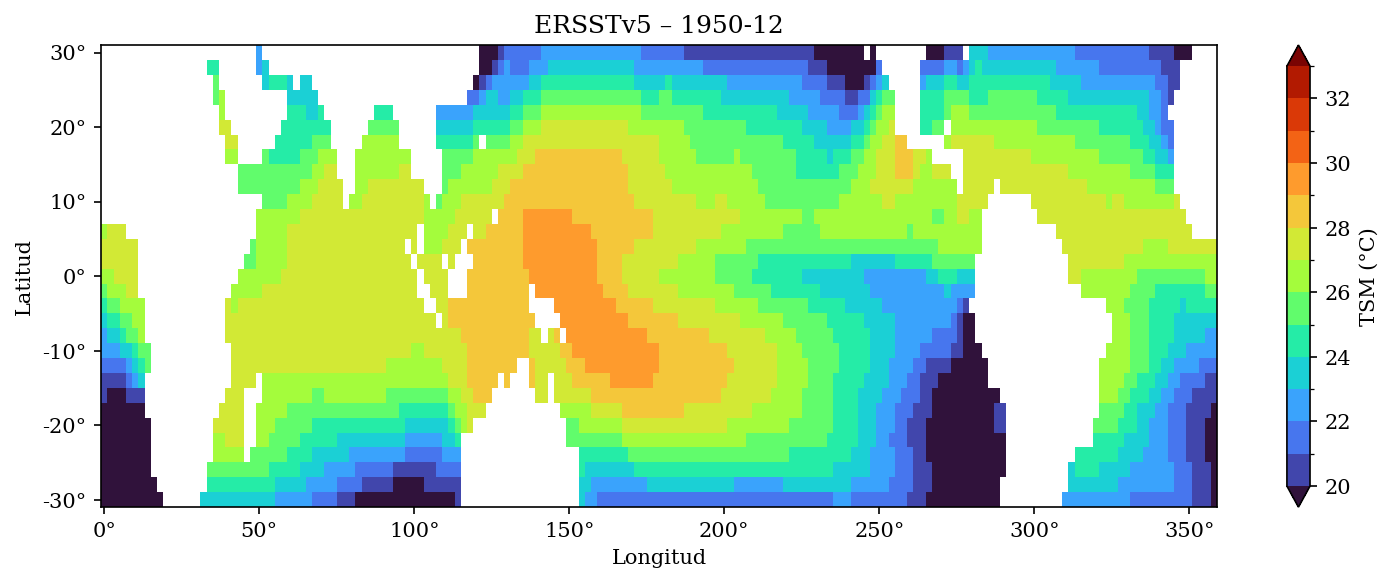
\includegraphics[width=\textwidth]{figuras/sst_2d_ERSSTv5.png}
\end{subfigure}
\begin{subfigure}[t]{0.75\textwidth}
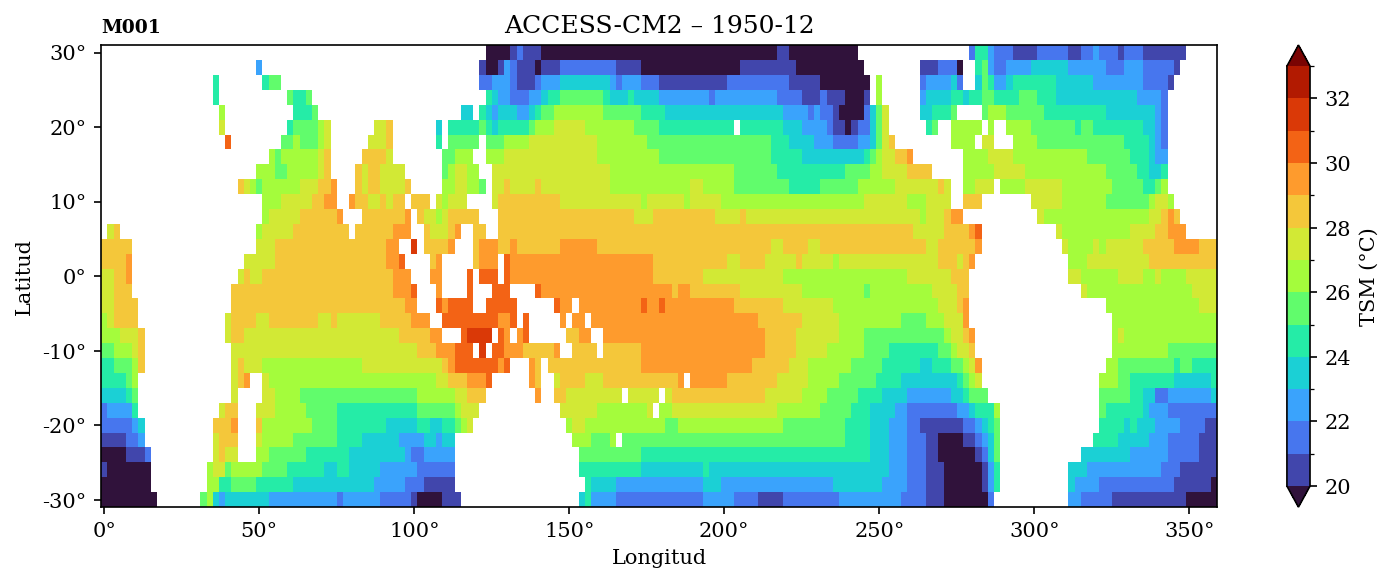
\includegraphics[width=\textwidth]{figuras/M001_sst_2d_ACCESS-CM2.png}
\end{subfigure}
\begin{subfigure}[t]{0.75\textwidth}
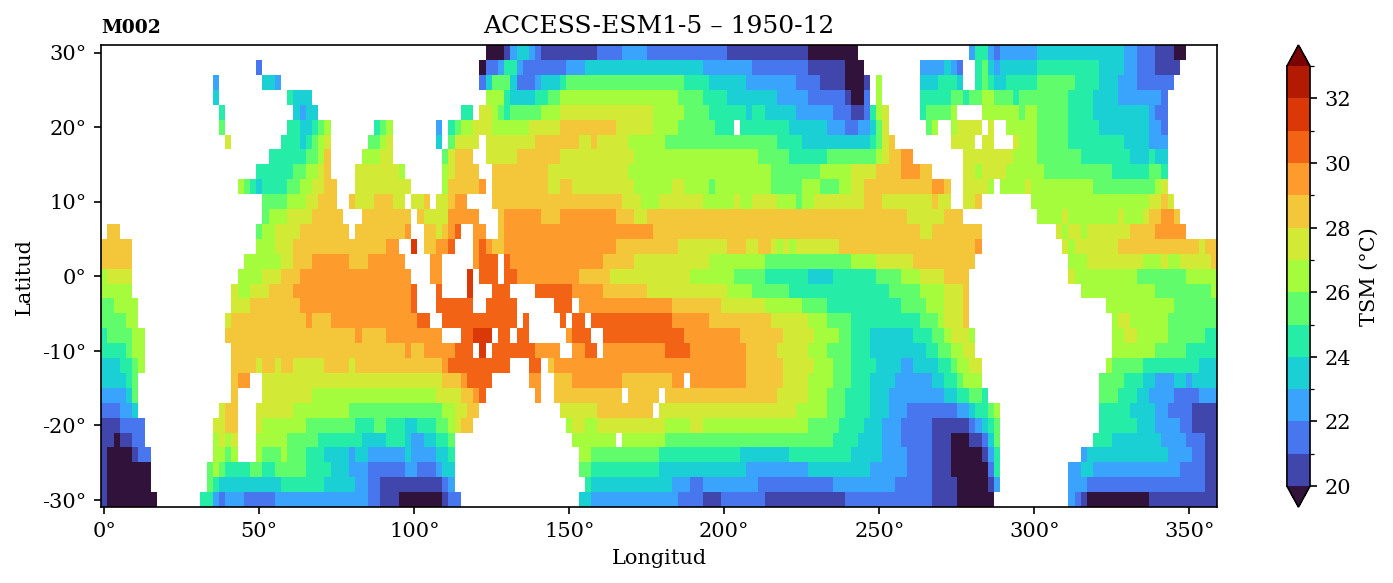
\includegraphics[width=\textwidth]{figuras/M002_sst_2d_ACCESS-ESM1-5.png}
\end{subfigure}
\begin{subfigure}[t]{0.75\textwidth}
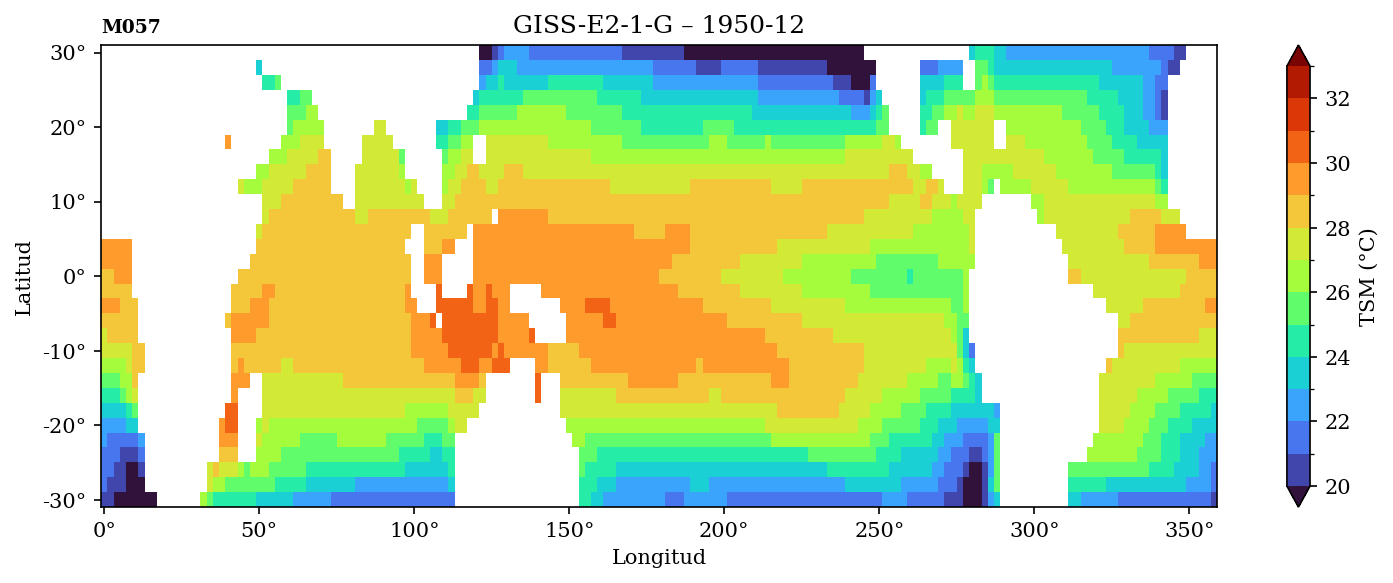
\includegraphics[width=\textwidth]{figuras/M057_sst_2d_GISS-E2-1-G.png}
\end{subfigure}
\caption[Campo de TSM de diciembre de 1950: ERSSTv5 y tres modelos de 250\,km.]{Temperatura superficial del mar de un mes de muestra (diciembre de 1950) en toda la ventana de descarga (0°--360°, 30°S--30°N), ya en la grilla, calendario, unidades y máscara océano-tierra comunes (Pasos~04--05). De arriba hacia abajo: ERSSTv5 y los modelos M001, M002 y M057 (Cuadro~\ref{tab:modelos}). Es una verificación visual de que todas las fuentes comparten grilla y máscara; al ser un mes aislado, no es una medida de desempeño.}
\label{fig:mapas2d}
\end{figure}

La Figura~\ref{fig:series} muestra la serie completa (\texttt{historical} y los tres escenarios SSP) de los mismos tres modelos en Niño~3.4, y la Figura~\ref{fig:boxplot} compara la distribución de la TSM histórica de ERSSTv5 y de los 40 modelos en ambas cajas.

\begin{figure}[htbp]
\centering
\begin{subfigure}[t]{\textwidth}
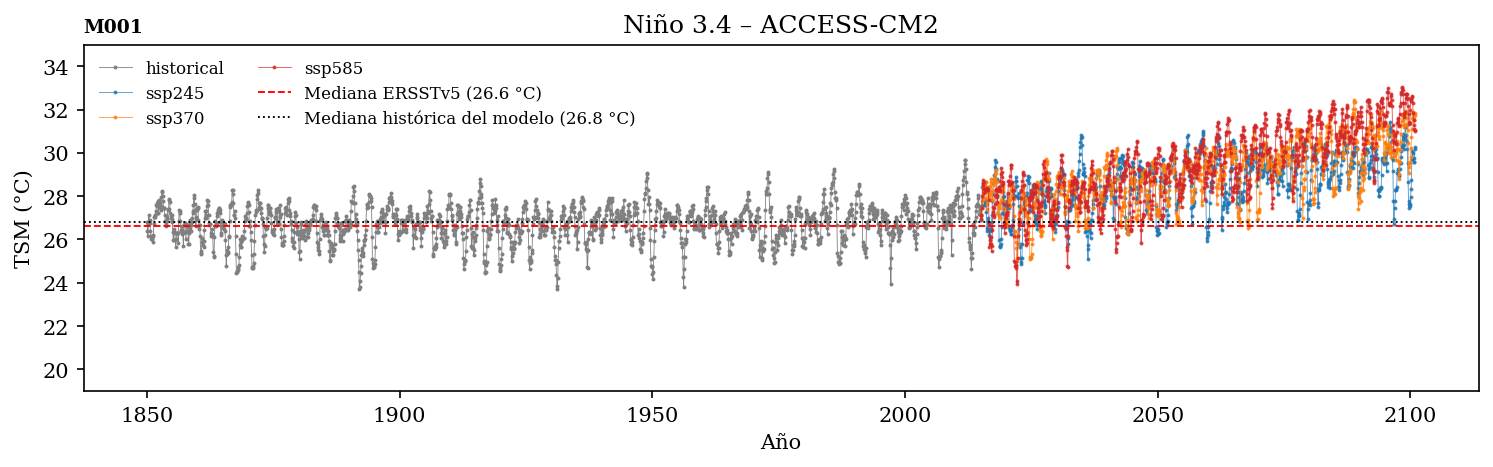
\includegraphics[width=\textwidth]{figuras/M001_serie_ACCESS-CM2_sst_Nino3.4.png}
\end{subfigure}
\begin{subfigure}[t]{\textwidth}
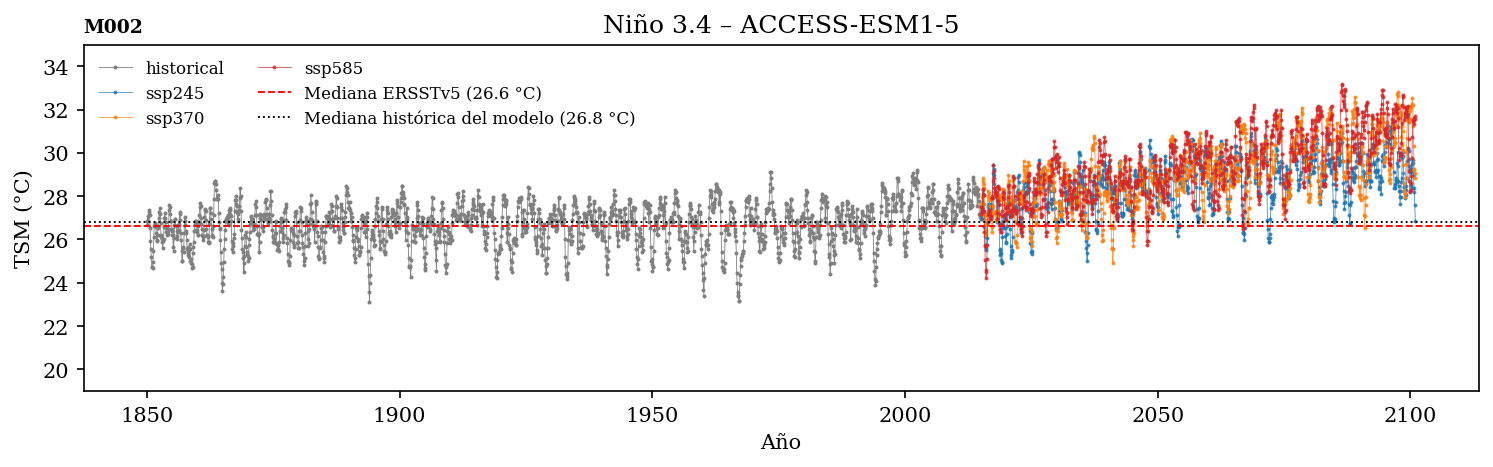
\includegraphics[width=\textwidth]{figuras/M002_serie_ACCESS-ESM1-5_sst_Nino3.4.png}
\end{subfigure}
\begin{subfigure}[t]{\textwidth}
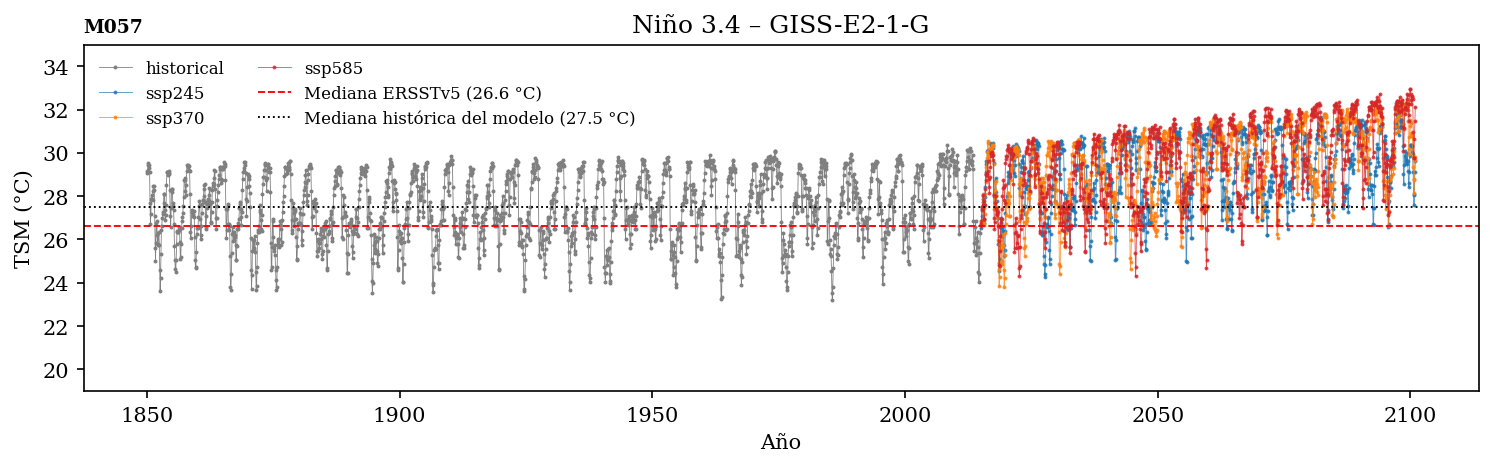
\includegraphics[width=\textwidth]{figuras/M057_serie_GISS-E2-1-G_sst_Nino3.4.png}
\end{subfigure}
\caption[Series de TSM en Niño~3.4 de tres modelos de 250\,km.]{TSM mensual promediada en Niño~3.4 (1850--2100): \texttt{historical} en gris y los tres escenarios SSP superpuestos, para los tres modelos de la Figura~\ref{fig:mapas2d}. Cada dato mensual se marca con un punto, sin interpolar huecos, de modo que un tramo sin puntos revelaría un hueco real de datos. Las líneas horizontales son la mediana de ERSSTv5 (roja, discontinua) y la mediana histórica del modelo (negra, punteada), ambas sobre el periodo común a las dos fuentes; su separación es el sesgo del modelo. El eje vertical es el mismo (19--35\,°C) en todos los paneles y en ambas cajas. Las series de Niño~1+2 se generan de la misma forma y se entregan junto con las demás figuras.}
\label{fig:series}
\end{figure}

\begin{figure}[htbp]
\centering
\begin{subfigure}[t]{\textwidth}
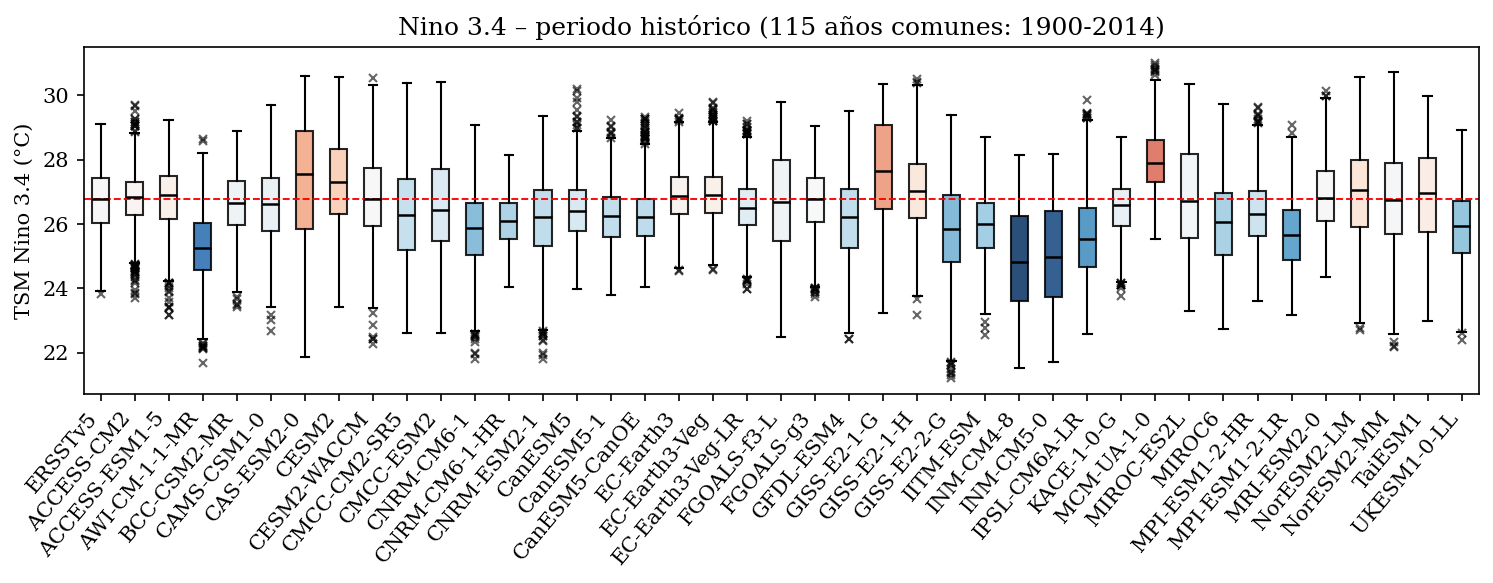
\includegraphics[width=\textwidth]{figuras/boxplot_Nino3.4.png}
\caption{Niño~3.4}
\end{subfigure}
\begin{subfigure}[t]{\textwidth}
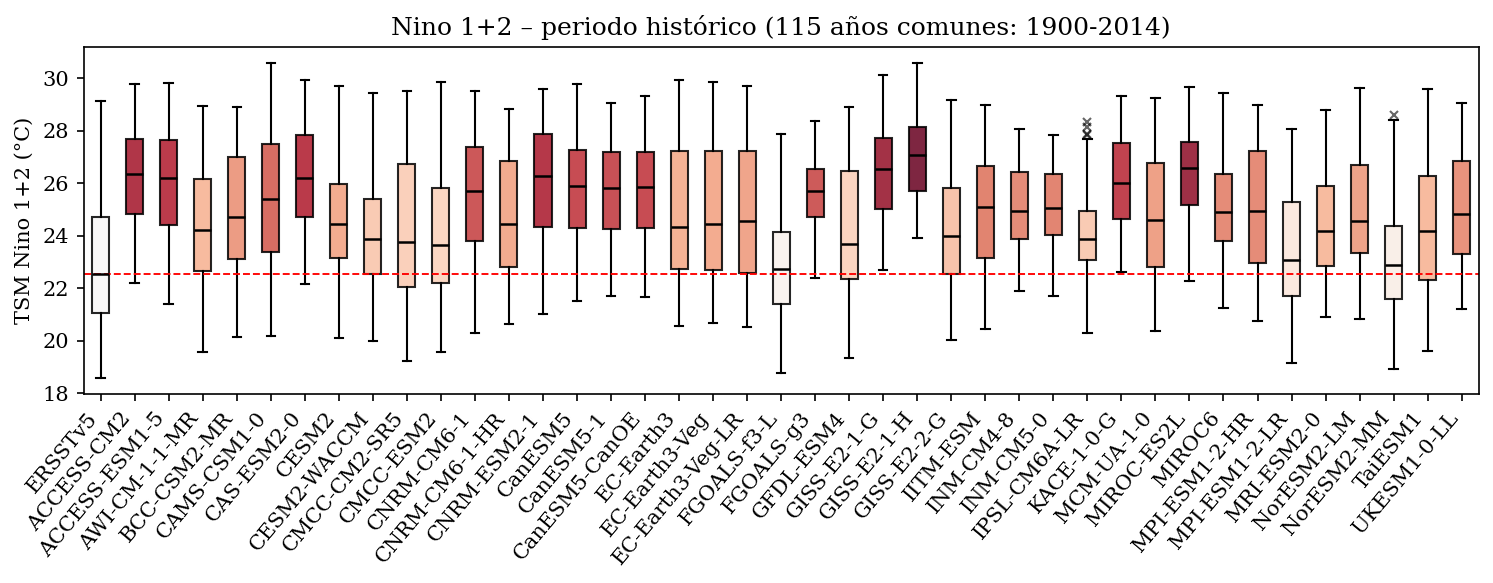
\includegraphics[width=\textwidth]{figuras/boxplot_Nino1+2.png}
\caption{Niño~1+2}
\end{subfigure}
\caption[Distribución de la TSM histórica en Niño~3.4 y Niño~1+2: ERSSTv5 frente a los 40 modelos.]{Distribución de la TSM mensual en cada caja para ERSSTv5 y los 40 modelos seleccionados, en el periodo común a todas las fuentes (1900--2014). Cada caja se colorea según la diferencia entre su mediana y la de ERSSTv5 (rojo, más cálido; azul, más frío); la línea roja discontinua marca la mediana observada.}
\label{fig:boxplot}
\end{figure}

Esta comparación preliminar ya anticipa un contraste entre cajas que el Entregable~2 deberá cuantificar. En Niño~3.4 la mediana de los modelos está cerca de la observada: 20 de los 40 modelos quedan a menos de 0{,}5\,°C de ERSSTv5 y el sesgo mediano es de $-0{,}24$\,°C. En Niño~1+2, 38 de los 40 modelos son más cálidos que la observación en más de 0{,}5\,°C, con un sesgo mediano de $+2{,}2$\,°C (rango de $+0{,}2$ a $+4{,}5$\,°C). Este sesgo cálido junto a la costa es coherente con lo señalado en la Sección~\ref{sec:similitudes} y con \citet{erickson2023}, quienes encuentran en la mayoría de los modelos CMIP6 un estado medio sesgado hacia condiciones de tipo El Niño, debido a sesgos cálidos de la TSM en el Pacífico tropical oriental. Refuerza la necesidad de reportar el sesgo de forma explícita y de calcular los índices como anomalías respecto de la climatología propia de cada modelo, de modo que el sesgo medio no se confunda con la variabilidad. La evaluación formal de desempeño (climatología, sesgos, diagrama de Taylor, índices ONI, RONI e ICEN) corresponde al Entregable~2.
